\chapter{基于深度相机的静态模型的采集与预处理}
 本文通过捕捉物体形变获取形变关键帧,然后根据关键帧相对于静态模型的相对形变构建形变子空间,
 这些工作都需要获取物体的静态模型作为参照。
 本章的目的就是获取一个物体静态三维模型,作为后续形变捕捉与形变子空间构建的输入。
\begin{figure}[h]
    \centering
    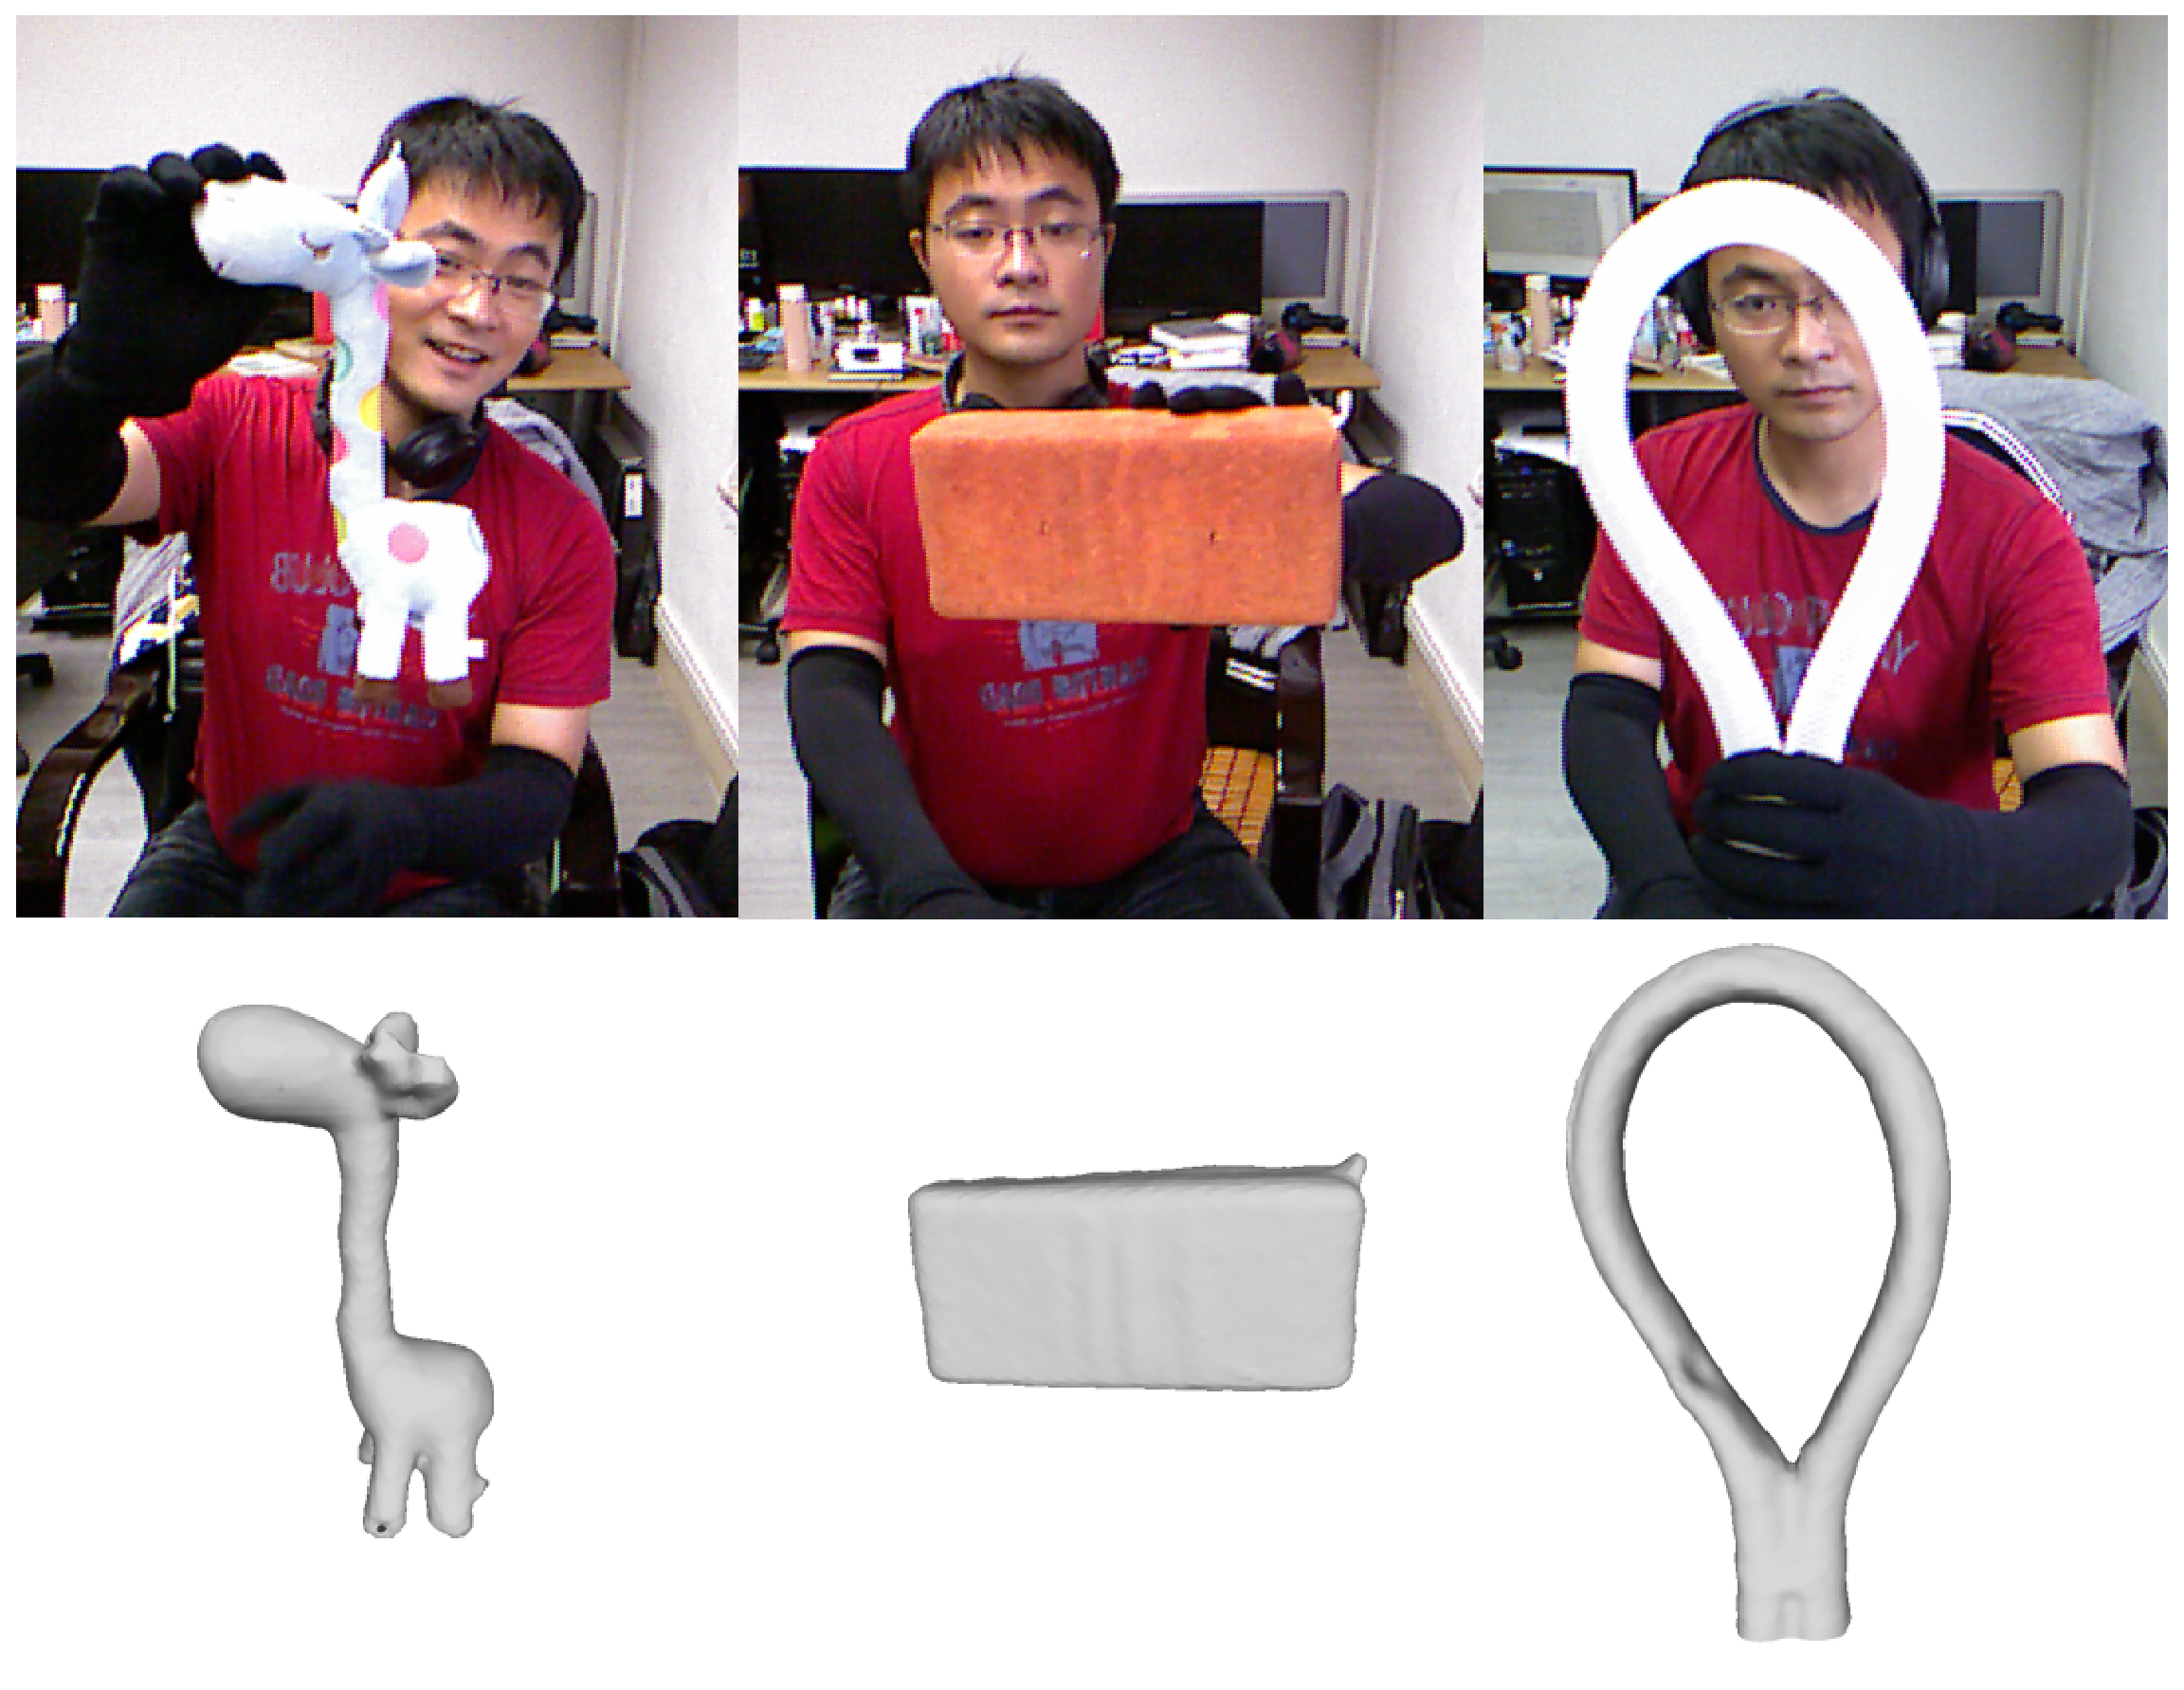
\includegraphics[width=0.9\textwidth]{./Pictures/static_mesh.eps}
    \caption{采集静态模型}
    \label{static_model}
\end{figure}

\section{基于深度相机的三维重建}
对于现实世界中存在的物体,其三维模型通常可以通过CAD软件建模或者借助扫描设备重建。
本文所使用的模型均借助深度相机重建。

深度相机是一种可以获取深度信息的设备,即能够测量物体表面距离相机的距离。
如同章节\ref{range_finding}所说,现在较为流行的三维测距技术有飞行时间、三角测距和结构光。
本文采用的是Microsoft生成的Kinect一代,这是一台基于结构光技术的深度相机。
Kinect除了能够获得RGB图像外,还能获得深度图像。
深度图像的每个像素记录的是物体表面距离相机的距离,
利用透视原理,可以推算出物体表面和相机的相对位置。
三维重建算法就可以通过扫描过程中获取的深度信息重建出物体的几何信息,获得三维模型。
本文采用的是KinectFusion算法\cite{izadi2011kinectfusion},
能够实时的借助深度相机重建三维模型。
KinectFusion算法\cite{izadi2011kinectfusion}以深度视频(由深度图像组成的图像流)为输入。
对于每一帧,会计算物体和相机的相对位置(物体在相机坐标系中的位置)
以及相机在世界坐标系(通常是第一帧的相机坐标)中的位置,
并将每一帧获得的数据融合到一个统一的模型坐标系中,从而得到三维模型。


